\chapter{Experiment Results}
\label{chapter:experiments}

\section{Dataset preparation}
\label{sec:dataset}
For conducting experiments on Compositional zero-shot image generation, we utilized several datasets, including publicly available datasets and ones we generated ourselves. In the initial stages to validate the feasibility of our ideas, we started with a very simple dataset that we generated ourselves. After achieving success on this dataset, we proceeded to use publicly available datasets. In the following sections, we will provide detailed introductions for each dataset.


\subsection{Shape Color Dataset}
\label{subsec:shapecolor}
This dataset is generated by the python OpenCV library, includes various geometric shapes of different colors.
\begin{itemize}
    \item \textbf{Two condition setting:} We use geometric shapes as the object category. There are a total of 6 object classes: Circle, Oval, Triangle, Rectangle, Pentagon, and Hexagon. We use color as the attribute category, with a total of 6 attribute classes: Red, Green, Blue, Yellow, Purple, and Black, resulting in a total of 36 compositions, As illustrated in table \ref{tab:twocondshape}. Each of them has 1000 training samples. Each training sample is a 64 * 64 pixel image, the size and the location of the geometric object are randomized.
    
    \begin{table} [H]
        \centering
        \begin{tabular}{c|c|c}
             & Condition 1 (Color) & Condition 2 (Geometric shape)\\
             \hline
             Labels & Circle, Hexagon, Oval, Pentagon, Rectangle, Triangle & Black, Blue, Green, Purple, Red, Yellow \\
        \end{tabular}
        \caption{Two condition setting of Shape Color dataset}
        \label{tab:twocondshape}
    \end{table}
    
    \item \textbf{Three condition setting:} Continuing with the two-condition setting, we use the size of the objects as a new category, with a total of 3 classes: Big, Medium, Small. This results in a total of 108 compositions, As illustrated in table \ref{tab:threecondzappo}. Each of them has 1000 training samples. Each training sample is a 64 * 64 pixel image.

    \begin{table} [H]
    \resizebox{\columnwidth}{!}{\begin{tabular} {c|c|c|c}
        \centering
             & Condition 1 (Size) & Condition 2 (Color) &  Condition 3 (Geometric shape)\\
             \hline
            Labels & Big, Medium, Small & Circle, Hexagon, Oval, Pentagon, Rectangle, Triangle & Black, Blue, Green, Purple, Red, Yellow \\
        \end{tabular}}
        \caption{Three condition setting of Shape Color dataset}
        \label{tab:threecondshape}
    \end{table}
\end{itemize}

\subsection{UT-Zappos50K}
The UT-Zappos50K dataset comprises a total of 50,025 images of footwear, categorized into four main types: Shoes, Boots, Slippers, and Sandals. These images are further divided based on their functional types. We have restructured the dataset and removed some ambiguous data in the dataset for our experiments, leaving us with 47,917 images for training.
\begin{itemize}
    \item \textbf{Two condition setting:} We retain the original four major categories as object category, introducing a new attribute category based on the presence or absence of heels, dividing it into two attribute classes: Heel and Flat. This results in a total of 8 compositions. As illustrated in table \ref{tab:twocondzappo}. 
    \begin{table} [H]
        \centering
        \begin{tabular}{c|c|c}
             & Condition 1 (Shoe height) & Condition 2 (Shoe type) \\
             \hline
             Labels & Heel, Flat & Boot, Shoe, Sandal, Slipper \\
        \end{tabular}
        \caption{Two condition setting of UT-Zappo50K dataset}
        \label{tab:twocondzappo}
    \end{table}
    \item \textbf{Three condition setting:} The images in the dataset were initially captured from a consistent perspective, so we horizontally flipped half of the data to introduce different shooting angles as a new category, with a total of 2 classes: Left, Right. Continuing with the two-condition setting, resulting a total of 16 compositions. As illustrated in table \ref{tab:threecondzappo}.
    \begin{table} [H]
        \centering
        \begin{tabular}{c|c|c|c}
             & Condition 1 (Filming angle) & Condition 2 (Shoe height) & Condition 3 (Shoe type)\\
             \hline
            Labels & Left, Right & Heel, Flat & Boot, Shoe, Sandal, Slipper \\
        \end{tabular}
        \caption{Three condition setting of UT-Zappo50K dataset}
        \label{tab:threecondzappo}
    \end{table}
\end{itemize}

\subsection{CelebFaces Attributes Dataset}
\label{subsec:celeba}
CelebFaces Attributes Dataset(CelebA) is a large-scale face attributes dataset with 202599 face images, each with 40 binray attribute annotations. 
\begin{itemize}
    \item \textbf{Two condition setting:}We use two of these attributes as our object category: Male and Female. For the attribute category, we use 4 of these attributes: Black Hair, Brown Hair, Blond Hair, Gray Hair. This results in a total of 8 compositions. As illustrated in table \ref{tab:twocondceleba}.
    \begin{table} [H]
        \centering
        \begin{tabular}{c|c|c}
             & Condition 1 (Hair color) & Condition 2 (Gender) \\
             \hline
             Labels & Black hair, Gray hair, Blond hair, Brown hair &  Male, Female \\
        \end{tabular}
        \caption{Two condition setting of CelebA dataset}
        \label{tab:twocondceleba}
    \end{table}
    \item \textbf{Three condition setting:}Continuing with the two-condition setting, we use hair style as a new category, dividing it into 2 classes: Wavy Hair and Straight Hair. This results in a total of 16 compositions. As illustrated in table \ref{tab:threecondceleba}
    
    \begin{table} [H]
        \centering
        \begin{tabular}{c|c|c|c}
             & Condition 1 (Hair style) & Condition 2 (Hair color) & Condition 3 (Gender)\\
             \hline
            Labels & Straight hair, Wavy hair & Black hair, Gray hair, Blond hair, Brown hair &  Male, Female \\
        \end{tabular}
        \caption{Three condition setting of CelebA dataset}
        \label{tab:threecondceleba}
    \end{table}
\end{itemize}



\section{Experiment setup}
\subsection{Training Diffusion model}
To train our model, we refer to the common hyperparameter settings of the stable diffusion model to configure the hyperparameters of our model. We used the following default hyperparameters: the training epoch was set to 100, the initial learning rate was set to $6 \times 10^{-5}$ with 10 warm-up epochs and the cosine learning rate scheduler was used for more stable training. For the optimization, we used AdamW optimizer with weight dacay values $10^{-4}$.

Diffusion process related hyperparameters are descride as follows. For the forward diffusion process, we set $T = 50$ for experiments with 2D Point Dataset, for the rest of experiments, we set $T = 1000$.For all experiments, the variance $\beta_T$ was set to $10^{-4}$ increasing linearly to 0.02. For the reverse process, we used classifier-free DDIM to sample images, the guildance strength $\omega$ to 1.8, $\eta$ was set to 0 and the samples were generated in 100 steps.

As for the hyperparameters related to the denoising models and the conditioner, they are described as the follows: For the denoising model used in 2D Point Dataset related experiments, we implemented the denoising model as a MultiLayer Perceptron (MLP) with three fully connected layers. For rest of the experiments, we implemented U-Net as our denoising model, we set the number of residual blocks to 2 in each downsample or upsample block. We set the base channel to 128 and the channel multiplier to [1, 2, 2, 2]. For the conditioner of cross attention , we used the same architecture in stable diffusion, which is a unmasked transformer, the number of attention head was set to 4 and the attention resolutions were set to [32, 16, 8].

The training images were all resized to 64 x 64 with RGB channels. All experiments were conducted on two NVIDIA Tesla V100 GPU.
The hyperparameter configuration for each architecture are illustrated with the following table.


\begin{table} [H]
    \centering
    \begin{tabular}{cc} 
         \hline
         & CCDM (with Conditioned ResBlock) \\
         \hline
         Diffusion steps & 1000\\
         Noise Schedule & linear \\
         Base Channels & 128 \\
         Number of Residual Blocks & 2\\
         Channel Multiplier & 1,2,2,2 \\
         Batch Size & 64 \\
         Epochs & 100 \\
         Learning Rate & $6 \times 10^{-5}$ \\
         Embedded Dimension & 512 \\
    \bottomrule[0.5mm]
    \end{tabular}
    \caption{Hyperparameters for CCDM(without attention) trained on the Shape Color Dataset, UT-Zappo50K, CelebA.}
    \label{tab:ccdmcondresblock}
\end{table}

\begin{table} [H]
    \centering
    \begin{tabular}{cc} 
         \hline
         & CCDM (with attention) \\
         \hline
         Diffusion steps & 1000\\
         Noise Schedule & linear \\
         Base Channels & 128 \\
         Number of Residual Blocks & 2\\
         Channel Multiplier & 1,2,2,2 \\
         Batch Size & 64 \\
         Epochs & 100 \\
         Learning Rate & $6 \times 10^{-5}$ \\
         Embedded Dimension & 512 \\
         \hline
         Number of Attention Heads & 4 \\
         CA-resolutions & 32, 16, 8 \\
         Transformer Depth & 1 \\
    \bottomrule[0.5mm]
    \end{tabular}
    \caption{Hyperparameters for CCDM(with attention) trained on the Shape Color Dataset, UT-Zappo50K, CelebA.}
    \label{tab:ccdmattention}
\end{table}

\subsection{Sampling}
During the generation phase, we utilize DDIM \cite{ho2020denoising} to accelerate the generation process. For each dataset, there is an unseen composition. We employ the trained CCDM to generate 1000 unseen compositional images using the unseen compositional class label. The hyperparameters used are illustrate in table \ref{tab:samplinghyperparameters}
\begin{table} [H]
    \centering
    \begin{tabular}{c|c}
        Hyperparameters & \\
        \hline
         Diffusion steps & 100\\
         Batch size & 200\\
         Guidance scale $\omega$ & 1.8\\
         Sampling stochasticity $\eta$ & 0\\
         Number of samples & 1000\\
    \end{tabular}
    \caption{Hyperparameters in sampling phase}
    \label{tab:samplinghyperparameters}
\end{table}

\subsection{Dataset splitting}
To train the binary classifiers within the image selector framework, we divided the available data into a training set and a validation set. We used 80 percent of the available data as the training set and 20 percent of the available data as the validation set. We used the training set to train the binary classifiers and tested them on the validation set.

\section{Evaluation Metrics}
Deep learning tasks require specific evaluation metrics that are tailored to the particular problem at hand. To evaluate the performance of CCDM, our focus is on the model's ability to generate unseen composition images. Therefore, we did not utilize the traditional Frechet Inception Distance(FID) \cite{heusel2017gans} for evaluation. During testing, the unseen composition images generated by CCDM are denoted as $N$, the unseen composition images selected by unseen image selector are denoted as $N_{select}$.
\begin{itemize}
    \item \textbf{Classification accuracy of binary classifier:} In order to assess whether the generated images by the model align with the description of unseen compositional class labels, we train a supervised binary classifier for each category class label of the unseen compositional class label. We evaluate the performance of each classifier based on its accuracy on the test dataset of each compositional class label.
    \item \textbf{Sample accuracy:} Follow \cite{liu2022compositional} evaluation metric, the images generated by CCDM are filtered by the image selector to choose those that match the unseen compositions. Sample accuracy is employed to assess CCDM's ability to generate unseen compositions, which includes whether the images generated by CCDM match the unseen compositional class label and the class label of each condition.
    \begin{equation}
        \text{Sample accuracy} = \frac{N_{select}}{N}
    \end{equation}
\end{itemize}


\section{Experiment results}
We designed various architectures for testing on each dataset, including both two-condition and three-condition settings. In this comparison, we evaluated different conditioning mechanisms and class encoder structures using sample accuracy. The detailed dataset settings are provided section \ref{sec:dataset} in  The detailed conditioning mechanisms are provided in figure \ref{fig:add}, figure \ref{fig:adagn}, figure \ref{fig:ic}, figure \ref{fig:ca}.

\subsection{Experiment results on shape color dataset}
After the successful experimentation with the 2D point dataset, we proceeded to test our model with more complex and higher-dimensional data, which is a major application of modern diffusion models:image generation. We began with our self-created shape color dataset \ref{subsec:shapecolor}, employing various architectures for the generation of unseen composition images. We designed different scenarios to assess the performance of CCDM

\begin{figure} [H]
    \centering
    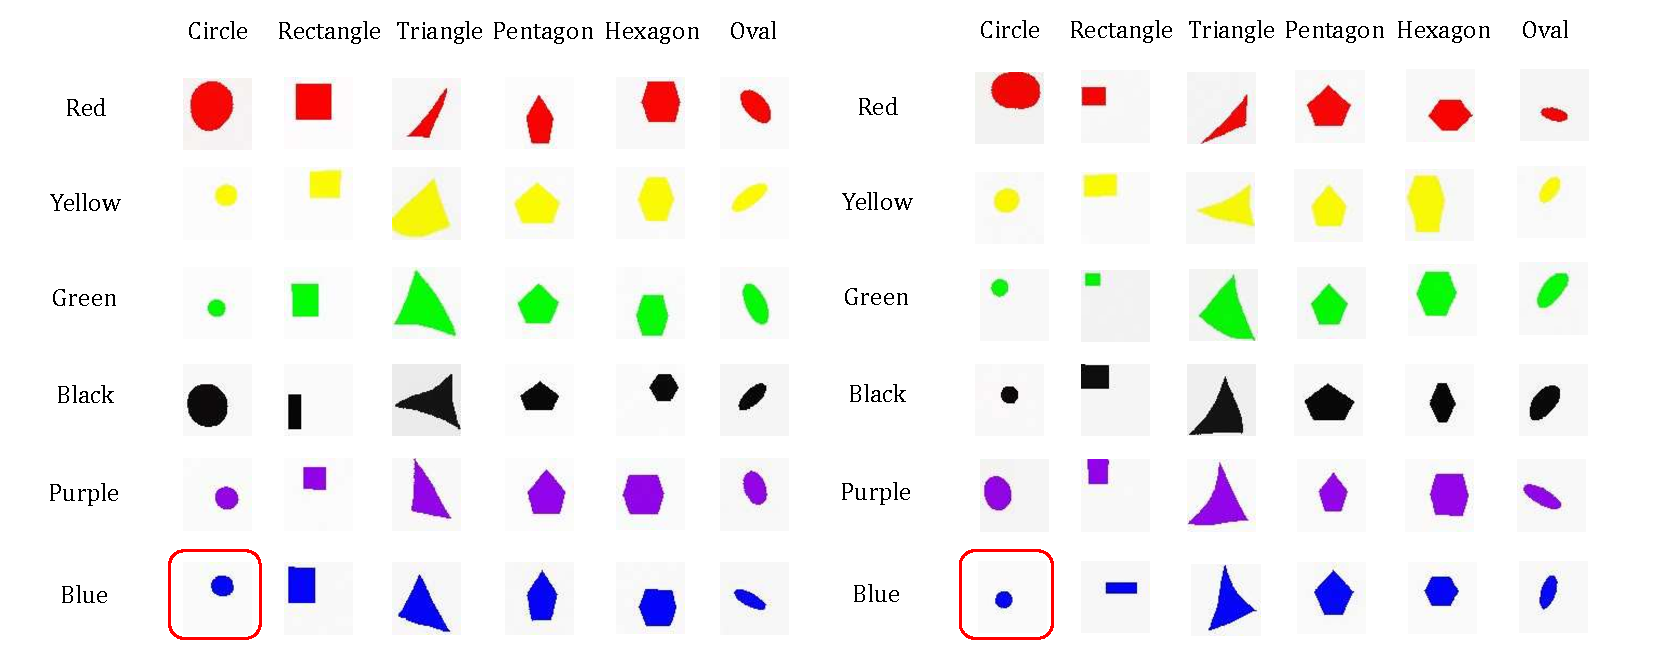
\includegraphics[width=1\linewidth]{figures/ShapeColor1.pdf}
    \caption{Under two condition setting of shape color dataset. Samples generated from CCDM, the unseen composition images are represented in red boxes.}
    \label{fig:sample_1}
\end{figure}

\begin{table} [H]
    \centering
    \begin{tabular}{cc}
         Classifier & Accuracy on validation set($\%$) $\uparrow$ \\
         \hline
         Blue classifier & 100 \\
         Circle classifier & 100 \\
         
    \end{tabular}
    \caption{Accuracy of binary classifiers within image selector(Two conditions setting)}
    \label{ShapeColorBinAcc}
\end{table}

\begin{table} [H]
    \centering
    \begin{tabular}{cccc}
         Architecture & $c_1$ accuracy $\uparrow$ & $c_2$ accuracy $\uparrow$ & All Corrects accuracy $\uparrow$ \\
         \hline
         Add & 0.54 & 0.55 & 0.31\\
         AdaGN & 0.46 & 0.76 & 0.35\\
         IC & 0.87 & \textbf{0.80} & \textbf{0.70}\\
         CA & \textbf{0.99} & 0.61 & 0.61\\
    \end{tabular}
    \caption{Architecture comparison on Shape Color Dataset (Two conditions setting)}
    \label{ShapeColorAcc}
\end{table}


\begin{figure} [H]
    \centering
    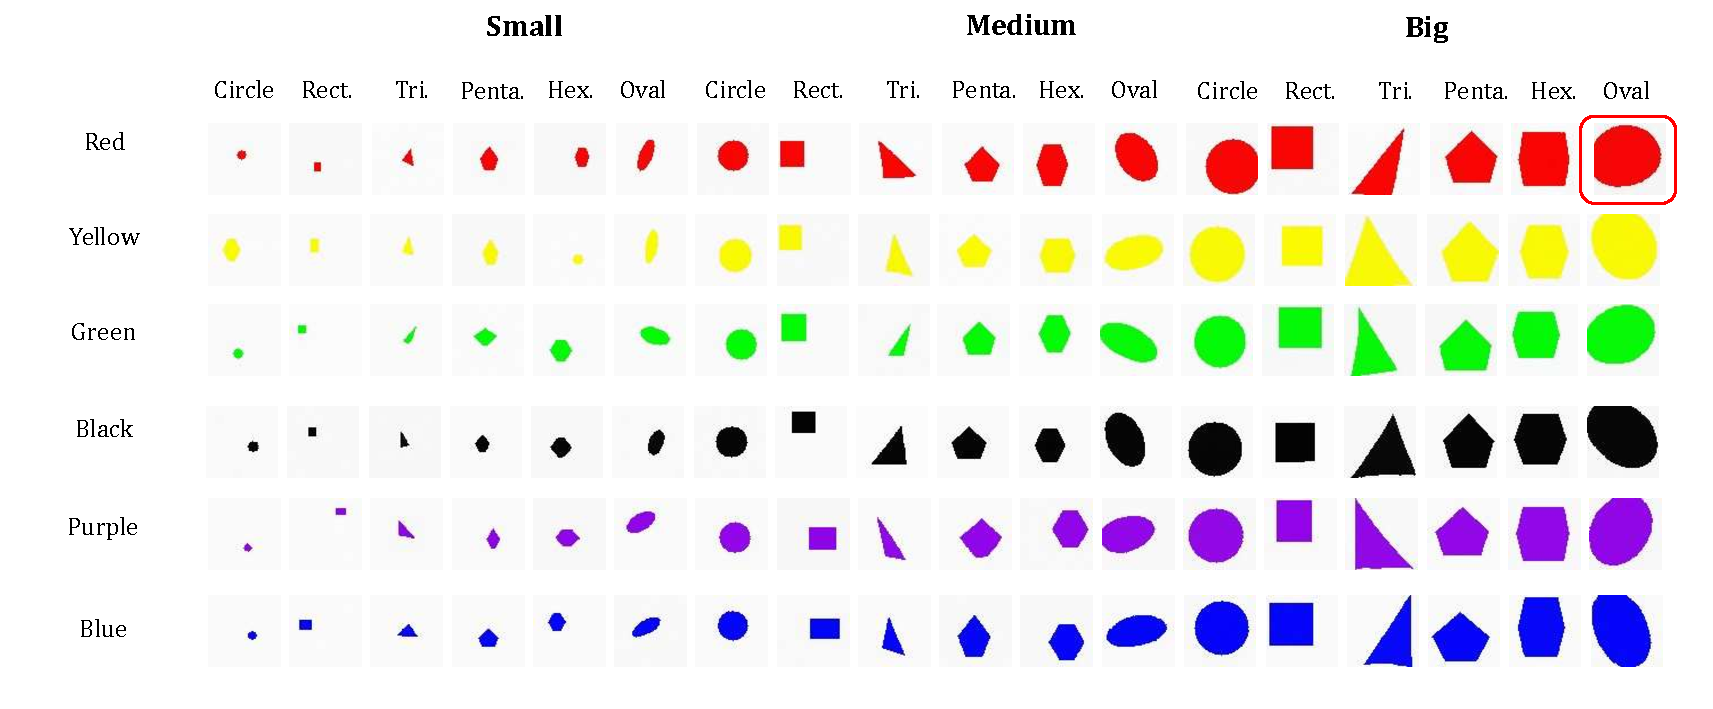
\includegraphics[width=1\linewidth]{figures/ShapeColor2.pdf}
    \caption{Samples of seen and unseen composition images generated from different architecture of CCDM, the unseen composition is represented by images enclosed in red boxes.}
    \label{fig:sample_3}
\end{figure}

From the experimental results in figure \ref{fig:sample_1} and figure \ref{fig:sample_3}, CCDM were able to successfully generate images of compositions that were not present during training. The results for seen compositions were also very promising across the board. These results also boosts our confidence in CCDM's ability to generalize to unseen compositions.

\begin{table} [H]
    \centering
    \begin{tabular}{cc}
         Classifier & Accuracy on validation set($\%$) $\uparrow$ \\
         \hline
         Big classifier & 100 \\
         Red classifier & 100 \\
         Oval classifier & 99.80 \\
    \end{tabular}
    \caption{Accuracy of binary classifiers within image selector(Three conditions setting)}
    \label{ShapeColorBinAccTri}
\end{table}

\begin{table} [H]
    \centering
    \begin{tabular}{ccccc}
         Architecture & $c_1$ accuracy $\uparrow$ & $c_2$ accuracy $\uparrow$ & $c_3$ accuracy $\uparrow$ & All Corrects accuracy $\uparrow$ \\
         \hline
         Add  & \textbf{1.0} & \textbf{1.0} & 0.98 & 0.98\\
         AdaGN & 0.99 & 0.99 & 0.96 & 0.95\\
         IC & \textbf{1.0} & \textbf{1.0} & \textbf{1.0} & \textbf{1.0}\\
         CA & \textbf{1.0} & 0.99 & \textbf{1.0} & 0.99\\
    \end{tabular}
    \caption{Architecture comparison on Shape Color Dataset (Three conditions setting)}
    \label{ShapeColorTriAcc}
\end{table}


\subsection{Experiment results on UT-Zappo50K}
After confirming that CCDM possesses the capability to generate unseen compositions, we proceeded to test CCDM on real-world datasets, specifically public datasets. We conducted tests on UT-Zappo50K, a common dataset in CZSL (Zero-Shot Learning), and made some modifications to the dataset structure. We examined CCDM's performance under different structures and scenarios. However, we encountered a challenge—instability in unseen composition generation. CCDM's ability to generate unseen composition images was not consistently stable under certain circumstances in these datasets. To address this, we employed an image selector to mitigate the issue. We will compare various architectures and evaluate their ability to generate unseen compositions. Detailed parameters of each architecture are provided in table \ref{tab:ccdmcondresblock}, table \ref{tab:ccdmattention}.

\begin{figure} [H]
    \centering
    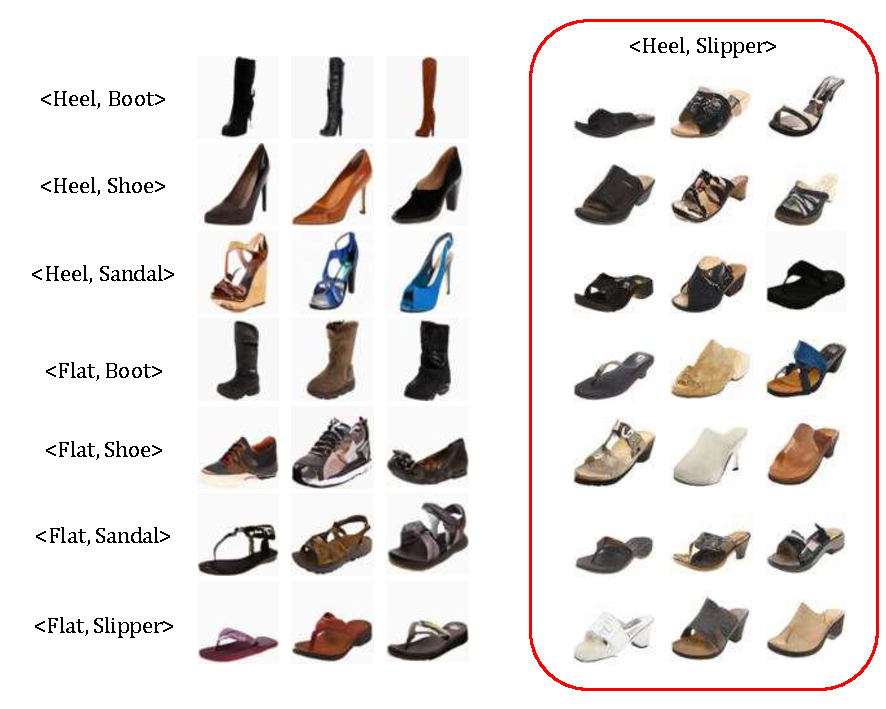
\includegraphics[width=1\linewidth]{figures/Zappo1.pdf}
    \caption{Under two condition setting of UT-Zappo50K. Samples generated from CCDM, the unseen composition images are represented in red boxes.}
    \label{fig:sample_6}
\end{figure}

\begin{table} [H]
    \centering
    \begin{tabular}{cc}
         Classifier & Accuracy on validation set($\%$) $\uparrow$ \\
         \hline
         Heel classifier & 87.50 \\
         Slipper classifier & 93.87 \\
         
    \end{tabular}
    \caption{Accuracy of binary classifiers within image selector(Two conditions setting)}
    \label{ZappoBinAcc}
\end{table}

\begin{table} [H]
    \centering
    \begin{tabular}{c|ccc}
         Architecture & $c_1$ accuracy $\uparrow$ & $c_2$ accuracy $\uparrow$ & All Corrects accuracy $\uparrow$ \\
         \hline
         Add & 0.17 & \textbf{0.9} & 0.07\\
         AdaGN & 0.28 & 0.71 & 0.06 \\
         IC & 0.31 & 0.86 & \textbf{0.18} \\
         CA & \textbf{0.62} & 0.50 & 0.16 \\
    \end{tabular}
    \caption{Architecture comparison on UT-Zappo50K Dataset (Two conditions setting)}
    \label{tab:Zappo50KAcc}
\end{table}


\begin{figure} [H]
    \centering
    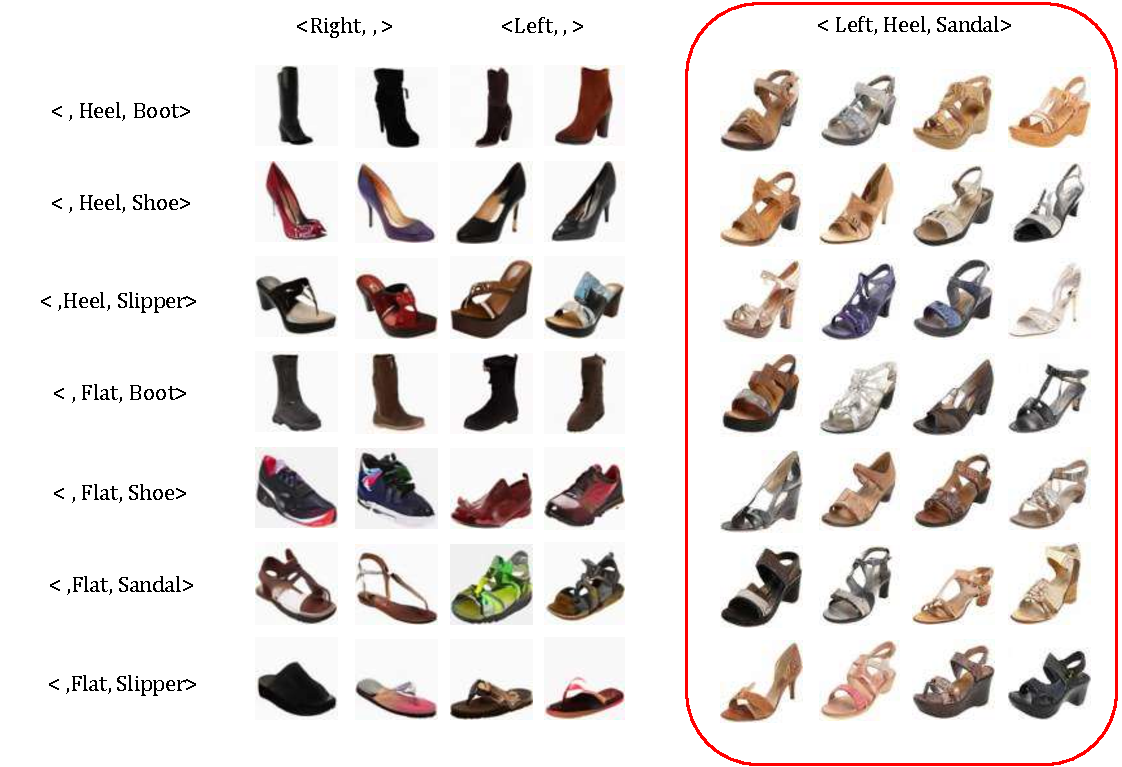
\includegraphics[width=1\linewidth]{figures/Zappo2.pdf}
    \caption{Under three condition setting of UT-Zappo50K. Samples generated from CCDM, the unseen composition images are represented in red boxes.}
    \label{fig:sample_8}
\end{figure}

\begin{table} [H]
    \centering
    \begin{tabular}{cc}
         Classifier & Accuracy on validation set($\%$) $\uparrow$ \\
         \hline
         Left classifier & 100 \\
         Heel classifier & 87.50 \\
         Sandal classifier & 95.60 \\
    \end{tabular}
    \caption{Accuracy of binary classifiers within image selector(Three conditions setting)}
    \label{ZappoBinAccTri}
\end{table}

\begin{table} [H]
    \centering
    \begin{tabular}{ccccc}
         Architecture & $c_1$ accuracy $\uparrow$ & $c_2$ accuracy $\uparrow$ & $c_3$ accuracy $\uparrow$ & All Corrects accuracy $\uparrow$ \\
         \hline
         Add  & \textbf{1.0} & 0.32 & 0.93 & 0.27\\
         AdaGN & \textbf{1.0} & 0.75 & 0.5 & \textbf{0.29}\\
         IC & \textbf{1.0} & 0.25 & \textbf{0.94} & 0.21\\
         CA & \textbf{1.0} & \textbf{0.99} & 0.06 & 0.06 \\
    \end{tabular}
    \caption{Architecture comparison on UT-Zappo50K Dataset (Three conditions setting)}
    \label{tab:Zappo50KTriAcc}
\end{table}

Figures \ref{fig:sample_6} and figure \ref{fig:sample_8} demonstrate CCDM's performance on the UT-Zappo50K dataset. It accurately generates unseen composition images, showcasing varied styles similar to real shoes. This illustrates CCDM's applicability to real-world datasets.In the results of table \ref{tab:Zappo50KAcc}, where $c_1$ represents "Heel," a subtle attribute, similar to the observations in table \ref{tab:CelebATriAcc}, we notice similar trends. In table \ref{tab:Zappo50KTriAcc}, where $c_2$ still represents "Heel" and $c_3$ represents "Sandal," we observe that Slipper and Sandal have many similarities in the UT-Zappo50K dataset. This leads to CCDM generating incorrect images, with many resembling slippers. Through experimentation, we confirm that CCDM possesses the capability of compositional zero-shot image generation. However, CCDM struggles with generating features that are subtle or have low separability, resulting in lower accuracy when generating such samples.


\subsection{Experiment results on CelebA}
To demonstrate that CCDM's ability to generate unseen compositions is not limited to a single case, we chose to conduct tests on the CelebA dataset, a well-known dataset in the field of image synthesis. CelebA Dataset is renowned for its comprehensive annotations, which facilitated a smoother experimental process. We selected several attributes from the original CelebA dataset to serve as different conditions, as detailed in \ref{subsec:celeba}. We conducted various tests on CCDM using different architectures and scenarios on the CelebA dataset.Detailed parameters of each architecture are provided in table \ref{tab:ccdmcondresblock}, table \ref{tab:ccdmattention}.

\begin{figure} [H]
    \centering
    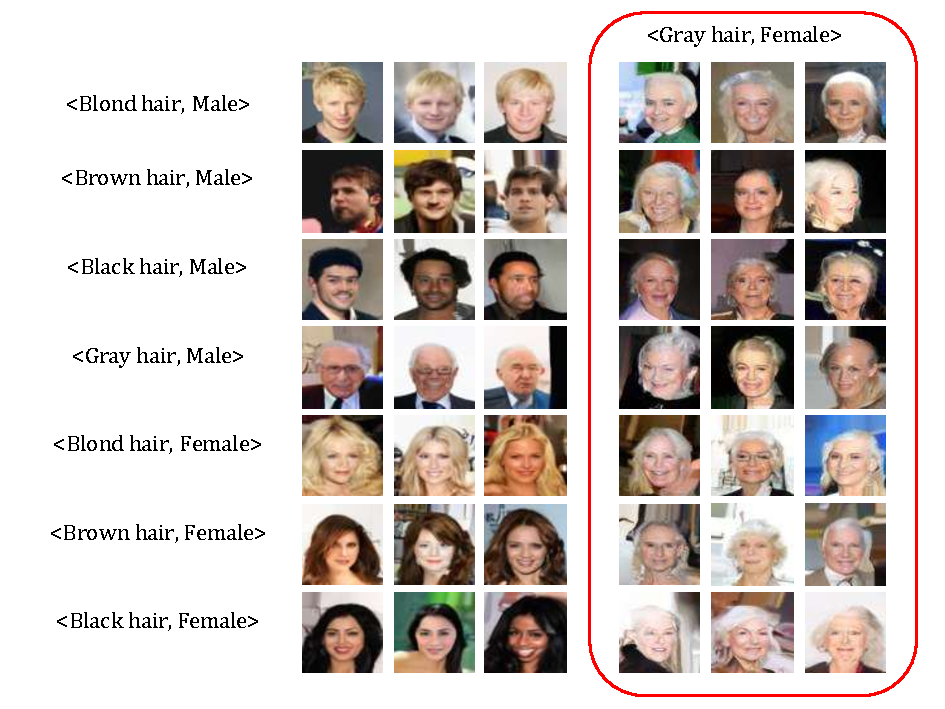
\includegraphics[width=1\linewidth]{figures/CelebA1.pdf}
    \caption{Under two condition setting of CelebA. Samples generated from CCDM, the unseen composition images are in red boxes.}
    \label{fig:sample_9}
\end{figure}

\begin{table} [H]
    \centering
    \begin{tabular}{cc}
         Classifier & Accuracy on validation set($\%$) $\uparrow$ \\
         \hline
         Gray hair classifier & 97.64 \\
         Female classifier & 99.12 \\
         
    \end{tabular}
    \caption{Accuracy of binary classifiers within image selector(Two conditions setting)}
    \label{CelebABinAcc}
\end{table}

\begin{table} [H]
    \centering
    \begin{tabular}{cccc}
         Architecture & $c_1$ accuracy $\uparrow$ & $c_2$ accuracy $\uparrow$ & All Corrects accuracy $\uparrow$ \\
         \hline
         Add  & 0.36 & 0.82 & 0.20\\
         AdaGN & \textbf{0.58} & 0.74 & \textbf{0.32}\\
         IC & 0.49 & 0.73 & 0.27 \\
         CA & 0.35 & \textbf{0.93} & 0.29 \\
    \end{tabular}
    \caption{Architecture comparison on CelebA Dataset (Two conditions setting)}
    \label{tab:CelebAAcc}
\end{table}

\begin{figure} [H]
    \centering
    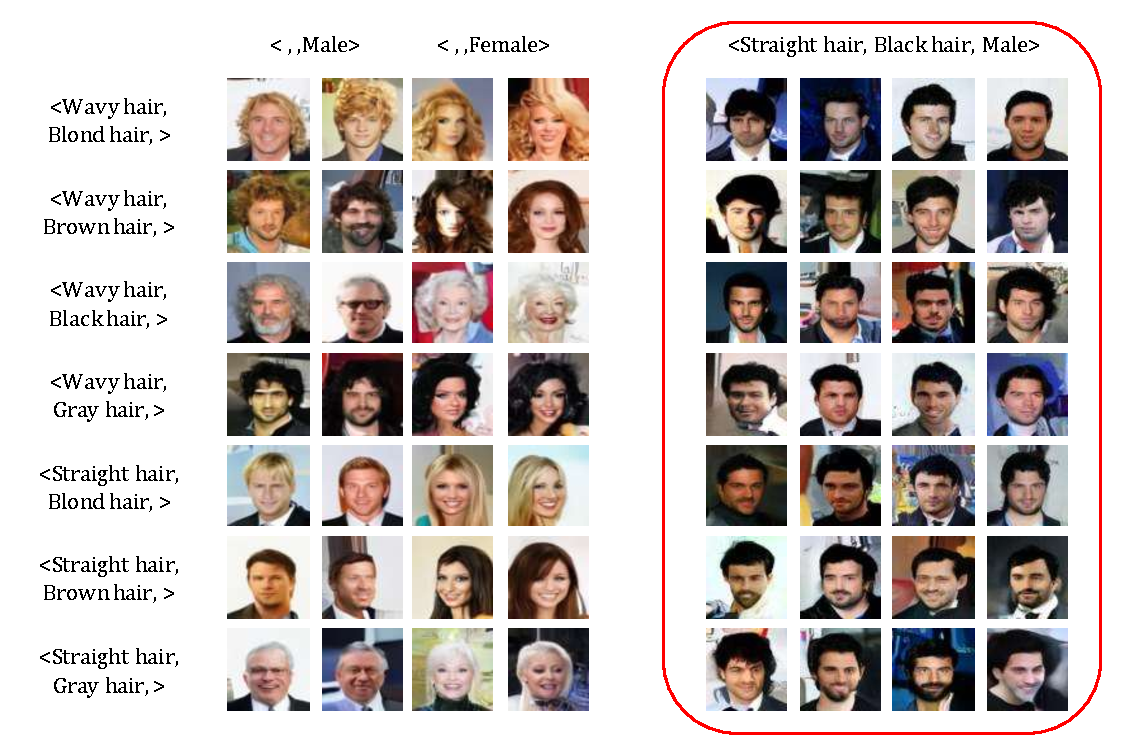
\includegraphics[width=1\linewidth]{figures/CelebA2.pdf}
    \caption{Under three condition setting of CelebA. Samples generated from CCDM, the unseen composition images are in red boxes.}
    \label{fig:sample_11}
\end{figure}

\begin{table} [H]
    \centering
    \begin{tabular}{cc}
         Classifier & Accuracy on validation set($\%$) $\uparrow$ \\
         \hline
         Straight hair classifier & 81.30 \\
         Black hair classifier & 100 \\
         Male classifier & 99.67 \\
    \end{tabular}
    \caption{Accuracy of binary classifiers within image selector(Three conditions setting)}
    \label{CelebABinAccTri}
\end{table}

\begin{table} [H]
    \centering
    \begin{tabular}{ccccc}
         Architecture & $c_1$ accuracy $\uparrow$ & $c_2$ accuracy $\uparrow$ & $c_3$ accuracy $\uparrow$ & All Corrects accuracy $\uparrow$ \\
         \hline
         Add  & \textbf{0.20} & 0.99 & 0.99 & \textbf{0.20}\\
         AdaGN & 0.11 & \textbf{1.0} & \textbf{1.0} & 0.11\\
         IC & \textbf{0.20} & 0.99 & \textbf{1.0} & 0.19\\
         CA & 0.06 & \textbf{1.0} & \textbf{1.0} & 0.06\\
    \end{tabular}
    \caption{Architecture comparison on CelebA Dataset (Three conditions setting)}
    \label{tab:CelebATriAcc}
\end{table}

In figure \ref{fig:sample_9} and figure \ref{fig:sample_11}, CCDM performs well on the CelebA dataset under the two-condition setting and three condition setting. However, the results generated by CCDM are not perfect. In table \ref{tab:CelebAAcc} and table \ref{tab:CelebATriAcc}, we compare the accuracy of generating unseen composition images using four different architectures. Although all can generate the unseen composition images correctly, the accuracy is not ideal. In the two-condition setting, where $c_1$ represents "Gray hair," this attribute has only a few samples in the dataset. In the three-condition setting $c_1$ represents "Straight hair", distinguishing between "Straight hair" and "Wavy hair" in male hair has low separability. We believe these factors contribute to the relatively low accuracy of CCDM in generating unseen composition images.

\section{Experiment analysis}
\begin{table} [H]
    \centering
    \begin{tabular}{cc}
         Architecture & Accuracy $\uparrow$\\
         \hline
         Add & 0.34\\
         AdaGN & 0.34\\
         IC & \textbf{0.42}\\
         CA & 0.36\\
    \end{tabular}
    \caption{Overall architecture comparison}
    \label{tab:OverallAcc}
\end{table}

Table \ref{tab:OverallAcc}  illustrates that among the four conditioning modules we used, Image Class Concatenation performs the best for compositional zero-shot image generation. This closely aligns with our expectations. For the diffusion model with compositional class labels as conditions, element-wise addition in the Addition module may aggregate information from multiple class labels, potentially hindering the model's ability to generate correct samples. The same rationale applies to AdaGN. Cross attention, when using compositional class label embeddings as keys and values, suffers from limited dimensions in both keys and values. Combined with the relatively insufficient data, it fails to fully exploit the power of cross attention. Concatenation, on the other hand, maximally preserves the information from compositional class embeddings. Additionally, concatenation avoids mixing the class embeddings of different conditions using addition, making it less prone to confusion for the model.


CCDM can achieve compositional zero-shot image generation across various datasets using the four architectures we employed. However, the quality of generated images is not consistently stable. We attribute this to not having found the most suitable conditioning module for compositional class labels yet. Nonetheless, the success on these datasets gives us confidence in using compositional class labels to guide the diffusion model. In future research, we aim to identify the optimal conditioning module for compositional class labels.
